\chapter{Preliminary analysis of \ac{AABW} samples}

\section{Introduction and Methods}
\begin{table}
\caption[\ac{AABW} samples used in the preliminary analysis]{Sampling time, location and physicochemical properties of \ac{AABW} samples used in this preliminary study.
All data were retrieved from the \ac{CTD} (SeaBird, Bellevue, USA) instrument used to collect the samples.}
\label{tab:deepsamples}
\smallskip
\begin{tabularx}{\textwidth}{llllXXXXXX}
\toprule
\textbf{Sample} & \textbf{Date} & \textbf{Latitude} & \textbf{Longitude} & \textbf{Sample Depth (m)} & \textbf{Temperature (\textdegree{}C)} & \textbf{Salinity (PSU)} & \textbf{Volume \linebreak filtered (L)}\\
\midrule

356 & 03/01/08 & $-66.7617$ & 144.4138 & 920 & $-1.9$ & 34.69 & 230\\
361 & 14/01/08 & $-66.4727$ & 140.5572 & 1170 & $-1.8$ & 34.56 & 225\\
365 & 23/01/08 & $-56.6967$ & 141.9125 & 3693 & 0.5 & 34.69 & 230\\
\bottomrule
\end{tabularx}
\end{table}

Three samples of \ac{AABW} were opportunistically obtained and analysed during the project described in \secreft{ch:polarfront}.
Two of these samples (356 and 361) were of newly formed \ac{AABW} waters on the Antarctic continental shelf, while one (365) was of abyssal \ac{AABW} from the South Australian basin \tabref{tab:deepsamples}.
DNA extraction, sequencing and construction of a taxonomic profile by \softwarename{blast} comparison to the RefSeq database were performed using the methods described in \secreft{ch:polarfront}.
A standardised and log-transformed Bray-Curtis resemblance matrix was constructed including the taxonomic profiles of the \ac{AABW} samples as well as the \ac{NZ} and \ac{SZ} samples described in \secreft{ch:polarfront}.
A \ac{nMDS} plot was then constructed from this matrix.
All statistical procedures were performed in \softwarename{PRIMER 6} as described by \citet{Clarke:2001ut}.

\section{Results and Discussion}

\begin{figure}
  \centering
  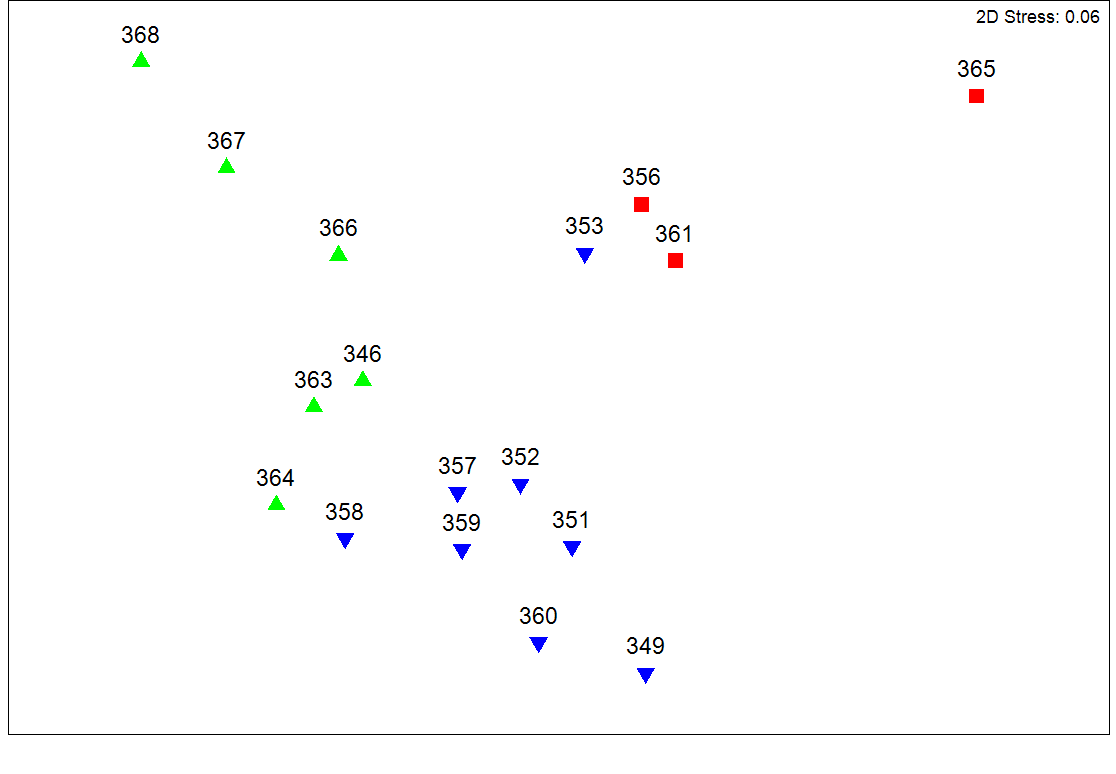
\includegraphics[width=\textwidth]{../biogeog/deepnmds.png}
  \caption[\ac{nMDS} of \ac{AABW}, \ac{NZ} and \ac{SZ} samples]{\ac{nMDS} plot showing distance between \ac{AABW}, \ac{NZ} and \ac{SZ} samples.
  Green triangles represent samples from the \ac{NZ}; blue inverted triangles from the \ac{SZ}; and red squares from \ac{AABW}.}
  \label{fig:deepnmds}
\end{figure}


Although the three \ac{AABW} samples were taken in deep, cold and aphotic waters \tabref{tab:deepsamples} compared to the surface \ac{AZ} and \ac{SZ} samples, the \ac{nMDS} plot suggested that the two continental shelf \ac{AABW} samples (356 and 361) were surprisingly similar to those of the \ac{AZ}, particularly sample 353 \figref{fig:deepnmds}.
